The SELECT statement is used to retrieve and display data from one or more tables.  The constructs in this section have the general form:

\ \   SELECT [ DISTINCT ]\ \ desired columns

\ \   FROM\ \ table

\ \ [ WHERE\ \ criteria for rows ]

\ \ [ ORDER BY\ \ Sorting sequence ]

\ \   ;

Only the first two clauses SELECT ... and FROM ... and the terminating  ;  are mandatory.



\begin{center}
  

\includegraphics[width=1.048cm,height=0.903cm]{images/img (2).png}

\end{center}
\begin{center}
\begin{minipage}{4.849cm}
   

\includegraphics[width=4.553cm,height=4.553cm]{images/img (14).png}
 

   

\includegraphics[width=1.582cm,height=0.674cm]{images/img (15).png}
 
\end{minipage}
\end{center}
Remember - anything in [brackets] is in option.

 (anything in [ ] is optional)

Selecting all the data from a single table: -

\ \ SELECT  *  FROM  table-name;

This will display all columns, ffor example:

\ \ SELECT \ \  * 

\ \  FROM \ \ \ \  EMP;

Displays all columns from the EMP table:

   
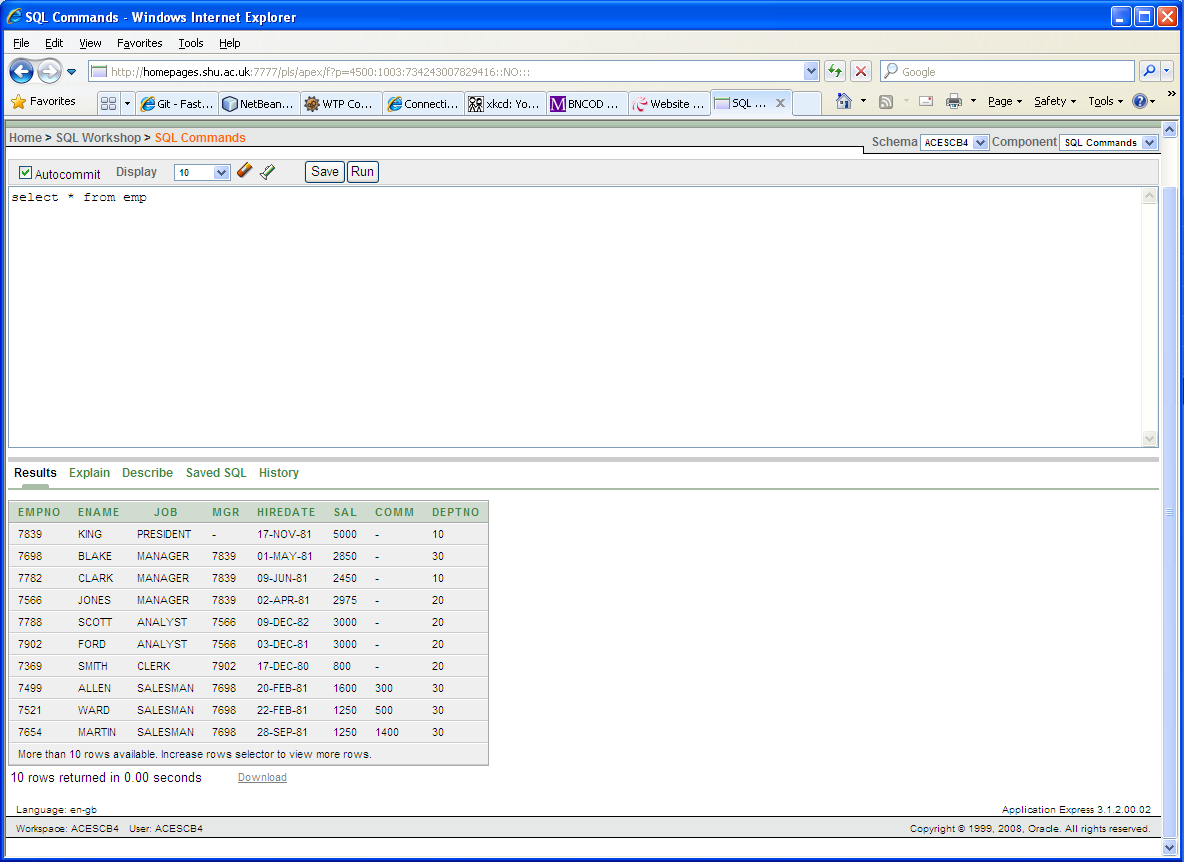
\includegraphics[width=14.785cm,height=7.089cm]{images/img (10).png}
 

The rows show in the same order as they were entered.

B1\ \ Display all the contents of the DEPT, EMP and SALGRADE tables.

\begin{flushleft}
\tablefirsthead{}
\tablehead{}
\tabletail{}
\tablelasttail{}
\begin{supertabular}{|m{14.405cm}|}
\hline
Select * from EMP ;\\\hline
Select\\\hline
Select\\\hline
\end{supertabular}
\end{flushleft}
To identify all your tables and views, use the special table, TAB

\ \ SELECT\ \ \ \  *

\ \ FROM\ \ \ \ \ \  TAB ;



\begin{center}
  
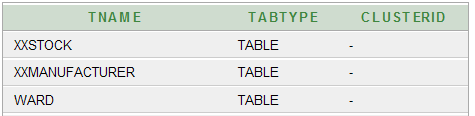
\includegraphics[width=12.298cm,height=2.992cm]{images/img (16).png}

\end{center}
To control which columns are displayed, and the order of them;-

\ \ SELECT  col1 [ , col2 ... ] FROM table-name;

Displays named columns.



\begin{center}
  

\includegraphics[width=1.076cm,height=0.917cm]{images/img (2).png}

\end{center}
There is a comma between each column name, but not after the final one.

For example, here are all employees with their employee number, name \& department number:

\ \ SELECT\ \ EmpNo,

\begin{center}
  
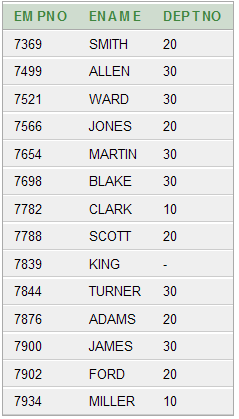
\includegraphics[width=5.826cm,height=5.6cm]{images/img (17).png}

\end{center}
\ \ \ \ \ \ Ename,

\ \ \ \ \ \ DeptNo

\begin{center}
  
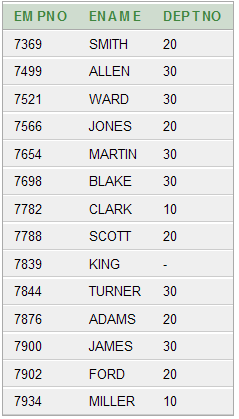
\includegraphics[width=5.826cm,height=4.662cm]{images/img (17).png}

\end{center}
\ \ FROM\ \ \ \ Emp ;

Below, REFNO NAME will would be displayed before NAME REFNO even though the table was first setup y were initially defined the other way round.  



\begin{center}
\begin{minipage}{5.191cm}
\begin{flushleft}
\tablefirsthead{}
\tablehead{}
\tabletail{}
\tablelasttail{}
\begin{supertabular}{|m{2.2389998cm}|m{2.55cm}|}
\hline
REFNO &
NAME\\\hline
A123 &
J Doe\\
A124 &
J Smith\\
B127 &
R Best\\
B128 &
J Best\\
C371 &
R Done\\\hline
\end{supertabular}
\end{flushleft}
\end{minipage}
\end{center}
SELECT\ \ REFNO,

\ \ \ \ NAME 

FROM\ \ \ \ \ \ \ \ CUST ;

For all the following exercises record the statement that will give you the required output.  Check against the given tables to ensure that the correct rows are selected and save the statements for future reference. 

(For each section the output from some of the queries is reproduced for you, but after that you are on your own!)

B2\ \ Display the name and commission of all the employees.



\begin{center}
  
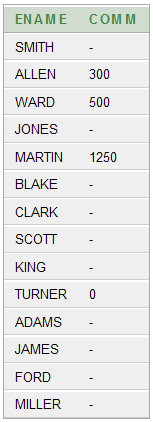
\includegraphics[width=3.281cm,height=4.748cm]{images/img (18).png}

\end{center}
\begin{center}
  
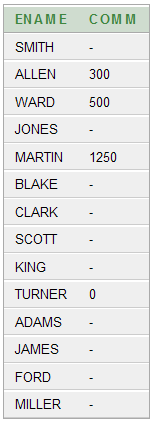
\includegraphics[width=3.27cm,height=4.12cm]{images/img (19).png}

\end{center}
\begin{flushleft}
\tablefirsthead{}
\tablehead{}
\tabletail{}
\tablelasttail{}
\begin{supertabular}{|m{7.051cm}|}
\hline
Select 

\\\hline
\end{supertabular}
\end{flushleft}
\subsection{}
\subsection{}
\subsection{}
B3\ \ Display the job title of all the employees.



\begin{center}
  
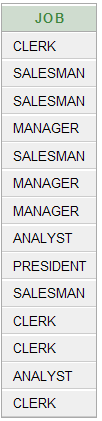
\includegraphics[width=2.42cm,height=4.623cm]{images/img (20).png}

\end{center}
\begin{center}
  
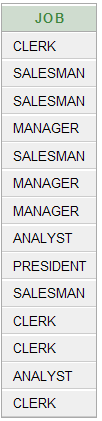
\includegraphics[width=2.431cm,height=5.398cm]{images/img (20).png}

\end{center}
\begin{flushleft}
\tablefirsthead{}
\tablehead{}
\tabletail{}
\tablelasttail{}
\begin{supertabular}{|m{8.0cm}|}
\hline
Select 

\\\hline
\end{supertabular}
\end{flushleft}
\subsection{Using DISTINCT}
It is not good practice to repeat values as part of the answer to such a question.  To remove duplicates within the result table, use the distinct keyword:

\ \ SELECT DISTINCT col1 [ , col2 ... ]  FROM  table-name ;

B4\ \ Display all the different job titles which currently exist in the company.

\begin{center}
  
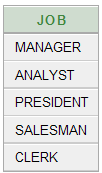
\includegraphics[width=2.491cm,height=4.124cm]{images/img (21).png}

\end{center}
\begin{flushleft}
\tablefirsthead{}
\tablehead{}
\tabletail{}
\tablelasttail{}
\begin{supertabular}{|m{11.537001cm}|}
\hline
Select 

\\\hline
\end{supertabular}
\end{flushleft}
\subsection{Simple calculations and column aliases}
It is also possible to manipulate the column values before displaying them: -



\begin{center}
\begin{minipage}{4.849cm}
   

\includegraphics[width=4.314cm,height=4.314cm]{images/img (22).png}
 

   

\includegraphics[width=1.582cm,height=0.674cm]{images/img (15).png}
 
\end{minipage}
\end{center}
\ \ SELECT\ \ col1 ,

\ \ \ \ \ \ col2*2.5 ,

\ \ \ \ \ \ col3+col4 AS alias1  {}-{}-  etc. note the column-renaming

\ \ FROM\ \ \ \ table-name ;

this displays specified columns, performs arithmetic on columns, and specifies an alias name to use as a column heading for the output.

For example, this:

SELECT\ \ ACCNO, BALANCE,

\begin{center}
\begin{minipage}{6.943cm}
\begin{flushright}
\tablefirsthead{}
\tablehead{}
\tabletail{}
\tablelasttail{}
\begin{supertabular}{|m{1.9909999cm}|m{2.299cm}|m{2.052cm}|}
\hline
ACCNO &
BALANCE &
BONUS\\\hline
1245890 &
\raggedleft 234.50 &
\raggedleft\arraybslash 23.45\\
1494315 &
\raggedleft 0.50 &
\raggedleft\arraybslash 0.05\\
5418490 &
\raggedleft 1789.40 &
\raggedleft\arraybslash 178.94\\\hline
\end{supertabular}
\end{flushright}
\end{minipage}
\end{center}
\ \ BALANCE * 0.1  AS BONUS

FROM\ \ ACC ;

Wouldill produce the result shown on the right.

B5\ \ Display the name and commission of all the employees together with another column that shows their commission increased by 10\%.  Use an appropriate column alias for the new column.



\begin{center}
  
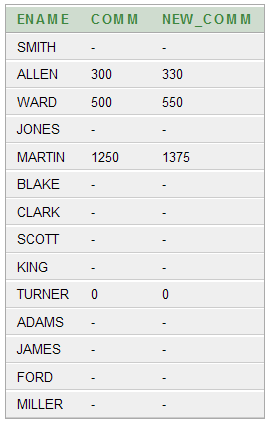
\includegraphics[width=7.17cm,height=6.218cm]{images/img (23).png}

\end{center}
\begin{flushleft}
\tablefirsthead{}
\tablehead{}
\tabletail{}
\tablelasttail{}
\begin{supertabular}{|m{6.8570004cm}|}
\hline
Select 

\\\hline
\end{supertabular}
\end{flushleft}
\subsection{The WHERE clause}
To SELECT specific rows from a single table the optional WHERE clause is used, for example:  Display all the customers in the Sheffield area:

\ \ SELECT *

\begin{center}
\begin{minipage}{9.192cm}
\begin{flushleft}
\tablefirsthead{}
\tablehead{}
\tabletail{}
\tablelasttail{}
\begin{supertabular}{|m{1.742cm}|m{1.798cm}|m{2.8cm}|m{2.049cm}|}
\hline
REFNO &
NAME &
ADDRESS &
AREA\\\hline
A123 &
J Doe &
1 High Street &
Sheffield\\
A124 &
J Smith &
2 West Street &
Sheffield\\
\end{supertabular}
\end{flushleft}
\end{minipage}
\end{center}
\ \ FROM CUST 

\ \ WHERE AREA = 'Sheffield' ;

WHERE is followed by an expression that will be either true or false (a Boolean). The simpler ones look like:

\begin{center}
\begin{minipage}{4.849cm}
   

\includegraphics[width=4.314cm,height=4.314cm]{images/img (24).png}
 

   

\includegraphics[width=1.582cm,height=0.674cm]{images/img (15).png}
 
\end{minipage}
\end{center}
Column  = Value

Value will be in quotes for text, but not for numbers, e.g.

AREA = 'Sheffield'

or

DEPTNO = 30

B6\ \ Display the employee number, name and current job of all those who work in Department 30.

\begin{center}
  
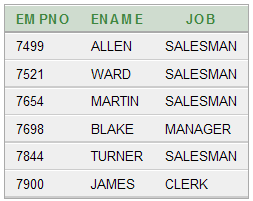
\includegraphics[width=4.9cm,height=3.861cm]{images/img (25).png}

\end{center}
\begin{flushleft}
\tablefirsthead{}
\tablehead{}
\tabletail{}
\tablelasttail{}
\begin{supertabular}{|m{9.202001cm}|}
\hline
Select 

From

Where\\\hline
\end{supertabular}
\end{flushleft}
B7\ \ Display the names of all the clerks, showing their employee number and that of their manager.  Note: strings are case sensitive and in single quote marks.

\begin{flushleft}
\tablefirsthead{}
\tablehead{}
\tabletail{}
\tablelasttail{}
\begin{supertabular}{|m{14.303cm}|}
\hline
Select 

\\\hline
\end{supertabular}
\end{flushleft}
\emph{As well as = other comparison operators are allowed: {\textless} ; {\textless}= ; {\textgreater} ;  {\textgreater}= ; {\textless}{\textgreater} and !=}

(!= and {\textless}{\textgreater} both mean not equal; do you know all the others?)

B8\ \ Display details of all employees whose commission is greater than salary.

\begin{flushleft}
\tablefirsthead{}
\tablehead{}
\tabletail{}
\tablelasttail{}
\begin{supertabular}{|m{14.303cm}|}
\hline
Select 

\\\hline
\end{supertabular}
\end{flushleft}
We can also use calculations involving columns in the comparisons, just as we do to display calculations

B9\ \ Display name, a twentieth of salary as 'Twentieth' and commission of all employees whose commission is greater than a twentieth of their salary.

\begin{flushleft}
\tablefirsthead{}
\tablehead{}
\tabletail{}
\tablelasttail{}
\begin{supertabular}{|m{14.303cm}|}
\hline
Select 

\\\hline
\end{supertabular}
\end{flushleft}
True or false expressions can be combined with logical operators AND, OR:

WHERE Exp1 OR Exp2

WHERE Exp1 AND Exp2



\begin{center}
  

\includegraphics[width=1.06cm,height=0.903cm]{images/img (2).png}

\end{center}
The AND and OR operators combine Boolean expression together. So this doesn't work:



\begin{center}
  

\includegraphics[width=1.443cm,height=1.427cm]{images/img (26).png}

\end{center}
SELECT  *

FROM  emp

WHERE deptno = 30 OR 40;

These do:

SELECT  *

\begin{center}
  

\includegraphics[width=1.443cm,height=1.184cm]{images/img (27).png}

\end{center}
FROM  emp

WHERE deptno = 30 OR deptno = 40;

SELECT  *

\begin{center}
  

\includegraphics[width=1.443cm,height=1.184cm]{images/img (27).png}

\end{center}
FROM  emp

WHERE deptno = 30 AND job = `MANAGER';

B10\ \ Display details of all clerks and analysts.  

\begin{flushleft}
\tablefirsthead{}
\tablehead{}
\tabletail{}
\tablelasttail{}
\begin{supertabular}{|m{14.303cm}|}
\hline
Select 

\\\hline
\end{supertabular}
\end{flushleft}
B11\ \ Display details of all clerks, analysts and salesmen.

\begin{flushleft}
\tablefirsthead{}
\tablehead{}
\tabletail{}
\tablelasttail{}
\begin{supertabular}{|m{14.303cm}|}
\hline
Select 

\\\hline
\end{supertabular}
\end{flushleft}
The operator NOT can be used in front of a Boolean:

WHERE NOT Exp;



\begin{center}
  

\includegraphics[width=1.06cm,height=0.903cm]{images/img (2).png}

\end{center}
The NOT operator is placed in front of a Boolean expression. So this doesn't work:



\begin{center}
  

\includegraphics[width=1.443cm,height=1.427cm]{images/img (26).png}

\end{center}
SELECT  *

FROM  emp

WHERE deptno = NOT 30;

These do:

SELECT  *

\begin{center}
  

\includegraphics[width=1.443cm,height=1.184cm]{images/img (27).png}

\end{center}
FROM  emp

WHERE NOT deptno = 30;

SELECT  *

\begin{center}
  

\includegraphics[width=1.443cm,height=1.184cm]{images/img (27).png}

\end{center}
FROM  emp

WHERE deptno != 30;

\ \ \ \ \ \ \ \ Remember that != is the 'not equal' operator 

B12\ \ Display details of employees who are neither managers nor president; you must not use knowledge about other jobs that might exist.

\begin{flushleft}
\tablefirsthead{}
\tablehead{}
\tabletail{}
\tablelasttail{}
\begin{supertabular}{|m{14.303cm}|}
\hline
Select 

\\\hline
\end{supertabular}
\end{flushleft}
There are several more useful construct and operators for Boolean expressions:

WHERE Value1 [ NOT ] BETWEEN Value2 AND Value3

WHERE Value  [ NOT ] IN (Value1 [ , Value2 , ... ] )

WHERE Value   [ NOT ] LIKE '\%charstring\%{}'

(\% means skip 0 to n characters) 

WHERE Value  [ NOT ] LIKE 'string1\_string2{}'

( \_ means for one and only one character)

WHERE Value IS [ NOT ] NULL

(The action of the BETWEEN, IN, LIKE and IS operators can be negated by NOT. Note that in these the case of constructs{}'IS NOT NULL', exceptionally, you can position the NOT operator as you would in English, rather than in front of the expression ).



\begin{center}
  

\includegraphics[width=1.06cm,height=0.903cm]{images/img (2).png}

\end{center}
To understand the constructs above takes more than this book. Refer to other material -- e.g. lectures - to work it out.

B13\ \ Display employee name, job and department number for employees whose names begin with `M'.

\begin{center}
\begin{minipage}{4.849cm}
   

\includegraphics[width=4.341cm,height=4.341cm]{images/img (28).png}
 

   

\includegraphics[width=1.582cm,height=0.674cm]{images/img (15).png}
 
\end{minipage}
\end{center}
\begin{flushleft}
\tablefirsthead{}
\tablehead{}
\tabletail{}
\tablelasttail{}
\begin{supertabular}{|m{11.493cm}|}
\hline
 Select 

\\\hline
\end{supertabular}
\end{flushleft}
B14\ \ Find a second way of answering B11 (details of all clerks, analysts and salesmen). Your solution must not use knowledge about other jobs that might exist.

\begin{flushleft}
\tablefirsthead{}
\tablehead{}
\tabletail{}
\tablelasttail{}
\begin{supertabular}{|m{12.782001cm}|}
\hline
Select 

\\\hline
\end{supertabular}
\end{flushleft}
B15\ \ Find a second way of answering B12 (employees who are neither managers nor president); again you must not use knowledge about other jobs that might exist. 

\begin{flushleft}
\tablefirsthead{}
\tablehead{}
\tabletail{}
\tablelasttail{}
\begin{supertabular}{|m{14.368cm}|}
\hline
Select 

\\\hline
\end{supertabular}
\end{flushleft}
B16\ \ Display details of employees who are not clerks, analysts or salesmen.  Write two different instructions to achieve this.

\begin{flushleft}
\tablefirsthead{}
\tablehead{}
\tabletail{}
\tablelasttail{}
\begin{supertabular}{|m{14.303cm}|}
\hline
Select 

\\\hline
Select 

\\\hline
\end{supertabular}
\end{flushleft}
B17\ \ Display details of employees whose salaries are between £1,200 and £1,400.  Write two different instructions to achieve this.

\begin{flushleft}
\tablefirsthead{}
\tablehead{}
\tabletail{}
\tablelasttail{}
\begin{supertabular}{|m{14.303cm}|}
\hline
Select 

\\\hline
Select 

\\\hline
\end{supertabular}
\end{flushleft}
B18\ \ Display details of employees whose salaries are not between £1,200 and £1,400.  Write two different instructions to achieve this.  Ensure you check your results!

\begin{flushleft}
\tablefirsthead{}
\tablehead{}
\tabletail{}
\tablelasttail{}
\begin{supertabular}{|m{14.303cm}|}
\hline
Select 

\\\hline
Select 

\\\hline
\end{supertabular}
\end{flushleft}
B19\ \ Display details of those salesmen and managers in dept 30 whose salary is greater than or equal to £1,500.  Check your results carefully.

\ \ \ \ (Note: for logical operators - AND takes precedence over OR).

Complex instructions may be written and tested in stages, building the complexity with each step.

Stage 1: Display details of salesmen and managers.

\begin{flushleft}
\tablefirsthead{}
\tablehead{}
\tabletail{}
\tablelasttail{}
\begin{supertabular}{|m{14.303cm}|}
\hline
Select 

\\\hline
\end{supertabular}
\end{flushleft}
Stage 2: Display details of those salesmen and managers in Department 30.  Run the instruction and check your results.

\begin{flushleft}
\tablefirsthead{}
\tablehead{}
\tabletail{}
\tablelasttail{}
\begin{supertabular}{|m{14.303cm}|}
\hline
Select 

\\\hline
\end{supertabular}
\end{flushleft}
Stage 3: Display details of those salesmen and managers in dept 30 whose salary is greater than or equal to £1,500.  Check your results carefully.

\begin{flushleft}
\tablefirsthead{}
\tablehead{}
\tabletail{}
\tablelasttail{}
\begin{supertabular}{|m{14.303cm}|}
\hline
Select 

\\\hline
\end{supertabular}
\end{flushleft}
\subsection[The ORDER BY clause]{The ORDER BY clause}
The ORDER BY clause is used to control the display order of selected records

ORDER BY\ \ col1 [ , col2 ... ]\ \ \ \ (first by col1, then by col2, etc.)

ORDER BY\ \ col1  [ ASC {\textbar} DESC ]\ \ (by col1, ascending, or descending)

ORDER BY \ \ n ; \ \ \ \ \ \ \ \ (by the nth column)



\begin{center}
  

\includegraphics[width=1.076cm,height=0.917cm]{images/img (2).png}

\end{center}
Note: The default ordering is ascending.

Null values are always displayed first regardless of sort sequence.

B20\ \ Display the employee number, current job and salary of all those who work in Department 30, with the output in ascending salary order.  As before, you may wish to write and test your instruction in a number of stages.



\begin{center}
  
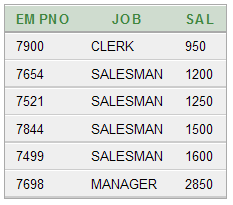
\includegraphics[width=5.514cm,height=4.835cm]{images/img (29).png}

\end{center}
\begin{flushleft}
\tablefirsthead{}
\tablehead{}
\tabletail{}
\tablelasttail{}
\begin{supertabular}{|m{9.482cm}|}
\hline
Select 

From

Where

Order By\\\hline
\end{supertabular}
\end{flushleft}


\begin{center}
\begin{minipage}{4.849cm}
   

\includegraphics[width=4.314cm,height=4.314cm]{images/img (22).png}
 

   

\includegraphics[width=1.582cm,height=0.674cm]{images/img (15).png}
 
\end{minipage}
\end{center}
B21\ \ Display the employee name and current job of all those who work in Department 30, with the output in descending salary order.

\begin{flushleft}
\tablefirsthead{}
\tablehead{}
\tabletail{}
\tablelasttail{}
\begin{supertabular}{|m{9.644cm}|}
\hline
Select 

\\\hline
\end{supertabular}
\end{flushleft}
Note: \ \ You were asked to order the rows using a column that is not selected for display; maybe a little unusual but not impossible.  How have you checked the accuracy of your result?

\begin{center}
  

\includegraphics[width=1.06cm,height=0.903cm]{images/img (2).png}

\end{center}
B22\ \ Display employee details for Departments 10 and 30, in name order, within each department.  Display the columns in the most appropriate order.

\begin{flushleft}
\tablefirsthead{}
\tablehead{}
\tabletail{}
\tablelasttail{}
\begin{supertabular}{|m{14.303cm}|}
\hline
Select 

\\\hline
\end{supertabular}
\end{flushleft}
B23\ \ Display the employee name, current job and salary of all those who work in Department 30, with the output in descending salary order within each job.

\begin{flushleft}
\tablefirsthead{}
\tablehead{}
\tabletail{}
\tablelasttail{}
\begin{supertabular}{|m{14.303cm}|}
\hline
Select 

\\\hline
\end{supertabular}
\end{flushleft}
The question asked for the selected data to be output in descending salary order within each job.  Does this influence the best order for displaying the columns?  Check the output of question B23 and suggest a better column order here.

\begin{flushleft}
\tablefirsthead{}
\tablehead{}
\tabletail{}
\tablelasttail{}
\begin{supertabular}{|m{14.303cm}|}
\hline
Select 

\\\hline
\end{supertabular}
\end{flushleft}
\subsection{}
\subsection{Dates}
Within Oracle, dates are stored and may be used just like any other number column.  To match or enter a date the value must be enclosed in single quote marks, dates may be in one of the formats:

\begin{center}
\begin{minipage}{4.849cm}
   

\includegraphics[width=4.341cm,height=4.341cm]{images/img (30).png}
 

   

\includegraphics[width=1.582cm,height=0.674cm]{images/img (15).png}
 
\end{minipage}
\end{center}
\ \ dd-mmm-yyyy  \ \ eg  {}'01-jan-2001'

\ \ dd/mmm/yyyy \ \ eg  {}'01/jan/2001' \ \ 

\ \ dd mmm yyyy \ \ eg  {}'01 jan 2001'

Without formatting, all dates will be displayed in the two-character year format dd-mmm-yy.



\begin{center}
  

\includegraphics[width=1.06cm,height=0.903cm]{images/img (2).png}

\end{center}
Avoid the two character date format: '01-jan-14' could be the year 14, instead of  2014.

B24\ \ Display details of employees recruited before 1st March 1981, in hire date order.  

\begin{flushleft}
\tablefirsthead{}
\tablehead{}
\tabletail{}
\tablelasttail{}
\begin{supertabular}{|m{14.303cm}|}
\hline
Select 

\\\hline
\end{supertabular}
\end{flushleft}
Date values can be compared using the same operators as numbers, and calculated on as if counting the number of days.

B25\ \ Display details of employees who were recruited during 1983.  Do NOT use wildcards.

\begin{flushleft}
\tablefirsthead{}
\tablehead{}
\tabletail{}
\tablelasttail{}
\begin{supertabular}{|m{14.303cm}|}
\hline
Select 

\\\hline
\end{supertabular}
\end{flushleft}
Oracle uses the variable SYSDATE for today's date. You should use this variable as you use column names.

SYSDATE is not, strictly speaking, todays date -- it is the system date on the Oracle server. The server could be in a different time zone, or poorly setup.

\begin{center}
  

\includegraphics[width=1.06cm,height=0.903cm]{images/img (2).png}

\end{center}
B26\ \ Display, in chronological order, the name, hire date and job details of employees who have been with the company for more than approximately 33 years.  Ensure the statement will work equally well today and in a month's time.  Do NOT pre-calculate any values you use. Hint: remember that dates are held and calculated on as a number of days.

\begin{flushleft}
\tablefirsthead{}
\tablehead{}
\tabletail{}
\tablelasttail{}
\begin{supertabular}{|m{14.303cm}|}
\hline
Select 

\\\hline
\end{supertabular}
\end{flushleft}
At times there will be no obvious table involved.  In such situations, Oracle provides the special table DUAL.

To display calculations:

\ \ SELECT 6 * 365 from DUAL ;

Test sysdate:

\ \ SELECT SYSDATE from DUAL ;

Or the current user:

\ \ SELECT USER from DUAL ;

B27\ \ Use Sysdate to display yesterday's date.

\begin{flushleft}
\tablefirsthead{}
\tablehead{}
\tabletail{}
\tablelasttail{}
\begin{supertabular}{|m{14.303cm}|}
\hline
SELECT 

FROM dual;

\\\hline
\end{supertabular}
\end{flushleft}
\clearpage